\documentclass{beamer}
\usepackage[utf8]{inputenc}
%\usepackage[brazil]{babel}
\usepackage{listings}

\usepackage{calc,alltt,amssymb,amsmath,latexsym,graphicx}
\usepackage{beamerthemesplit}

\lstset{basicstyle=\footnotesize,columns=fullflexible,frame=lines}

\title{GEGL}
\subtitle{Generic Graphics Library}
\author{Victor M. de Araujo Oliveira}
\date{\today}

\begin{document}

\begin{frame}
\titlepage
\begin{center}
  \resizebox{60mm}{!}{
\includegraphics{gegl.png}}
\end{center}
\end{frame}

\section[Contents]{}
\frame{\tableofcontents}

\section{Intro}

\subsection{Intro}

\begin{frame}
  \frametitle{What is it?}
GEGL is a graph based image processing framework.

GEGL's main purpose is to be the default way GIMP manipulate and
process images. But it can be used as a stand-alone lib as well.

  \begin{itemize}
    \item{Floating point images}
    \item{Supports many image formats}
    \item{Larger than RAM images (automatic disk swapping)}
    \item{Python, Ruby and Vala Bindings}
    \item{Lots of filters}
  \end{itemize}
\end{frame}

\subsection{How to Install}

\begin{frame}
  \frametitle{How to Install}
  
git clone git://git.gnome.org/gegl
\begin{itemize}
  \item{Ubuntu \\ sudo apt-get install gegl}
  \pause
  \item{./configure;make;sudo make install}
\end{itemize}
\end{frame}

\subsection{GEGL in GIMP}
\begin{frame}
\frametitle{GEGL in GIMP}
\{Open GIMP and introduce GEGL\}
\begin{itemize}
  \item{How to enable and use GEGL.}
  \item{Show and explain some filters.}
\end{itemize}
\end{frame}

\subsection{Tiled Buffers}

\begin{frame}
\frametitle{Tiled Buffers}
GEGL uses tiled buffers. This means some operations can be well-supported and others doesn't map well.
  \pause
  \begin{itemize}
    \item{Brightness-Contrast \pause \\ Processing a pixel only needs information about that pixel - OK}
    \pause
    \item{Blur \pause \\ Processing a pixel only needs information about that pixel and a fixed neighborhood around it - OK}
    \pause
    \item{Watershed \pause \\ Processing a pixel needs information from many others random ones - NO!}
  \end{itemize}
\end{frame}

\section{Processing Graph}

\subsection{Processing Graph}

\begin{frame}
\frametitle{Processing Graph}
\begin{center}
  \resizebox{110mm}{!}{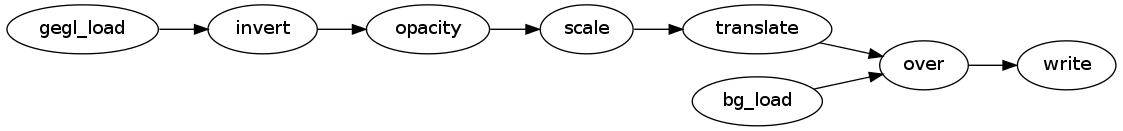
\includegraphics{ops/ops.png}}
\end{center}
Nodes represent operations in the image.

Edges link the output of a filter with the input of the next one.
\end{frame}

\begin{frame}
  \frametitle{Creating a Node}
  \lstinputlisting[firstline=35,lastline=39,language=C]{ops/test.c}
\end{frame}

\begin{frame}
  \frametitle{Linking nodes}
  \lstinputlisting[firstline=56,lastline=58,language=C]{ops/test.c}
  
  By default, the "output" attribute of a node is connected to the
  "input" of another one, but some nodes [like gegl:layer, gegl:over]
  can be have many input attributes.
\end{frame}

\begin{frame}
  \frametitle{Processing}
  \lstinputlisting[firstline=60,lastline=60,language=C]{ops/test.c}
  
  In order to evaluate 'write' node, GEGL evaluates all dependency nodes.
\end{frame}

\begin{frame}
  \frametitle{Some real code!}
  
  \{Let's see some GEGL code - ops/test.c\}
\end{frame}

\subsection{XML Description}

\begin{frame}
  \frametitle{XML Description}
  A Processing Graph can be described by a XML where tags are
  operations.
  
  \{Let's see an XML example - ops/test.xml\}
\end{frame}

\section{Python Bindings}

\begin{frame}
  \frametitle{Python Bindings}
  We can use GEGL in Python!
  
  Very useful to:
  \pause
  \begin{itemize}
    \item{Test composition of operations in an interactive way.}
    \pause
    \item{Use Python's flexive way to manipulate strings and XML files to generate custom filters.}
    \pause
    \item{GEGL can be easily used in the Python ecosystem [like a webserver that generates images according user data].}
    \pause
    \item{Infinite possibilities...}    
  \end{itemize}
\end{frame}

\begin{frame}
  \{Let's create the example from the previous section interactively in a Python shell\}
\end{frame}

\section{Operations}

\begin{frame}
\frametitle{Operations}

\begin{itemize}
\item{GeglOperationPointFilter}
\begin{itemize} \item{Brightness-Contrast} \item{Threshold} \item{Color-to-Gray} \end{itemize}
\item{GeglOperationAreaFilter}
\begin{itemize} \item{Motion Blur} \item{Sobel Edge Detection} \end{itemize}
\item{GeglOperationSource}
\begin{itemize} \item{Load Image} \end{itemize}
\item{GeglOperationSink}
\begin{itemize} \item{Save Image} \item{Display Image} \end{itemize}
\end{itemize}
\end{frame}

\begin{frame}
  \{Let's implement a Brightness-Contrast operation.\}
\end{frame}

\section{GSoC}

\begin{frame}
  \frametitle{GSoC - OpenCL in GEGL}

OpenCL (Open Computing Language) is a framework for
writing programs that execute across heterogeneous
platforms consisting of CPUs, GPUs, and other processors.

My proposal is about making possible to write GEGL plug-ins in OpenCL.
But the main point of the work is extending GeglBuffer to automatically
make the memory transferences between the CPU and GPU.

Also, I'm going to implementing some operations in OpenCL.
\end{frame}

\begin{frame}
\frametitle{Example of OpenCL code}

\lstinputlisting{opencl.cl}

\end{frame}

\section{Questions?}
\begin{frame}
  \frametitle{Questions?}
\end{frame}

\end{document}
